% \section{Circle}
% \subsection{Definition of circle}
% \subsubsection{Cartesian form}
% \begin{itemize}
%     \item $(x-a)^2+(y-b)^2=r^2$
% \end{itemize}

% \subsubsection{Parametric form}
% \begin{itemize}
%     \item $x=a+r\cos\theta$
%     \item $y=b+r\sin\theta$
% \end{itemize}

% \subsubsection{Polar form}
% \begin{itemize}
%     \item $r=a$
%     \item $r=a\sin\theta$
%     \item $r=a\cos\theta$
% \end{itemize}

\section{Parabola}
\subsection{Graph}
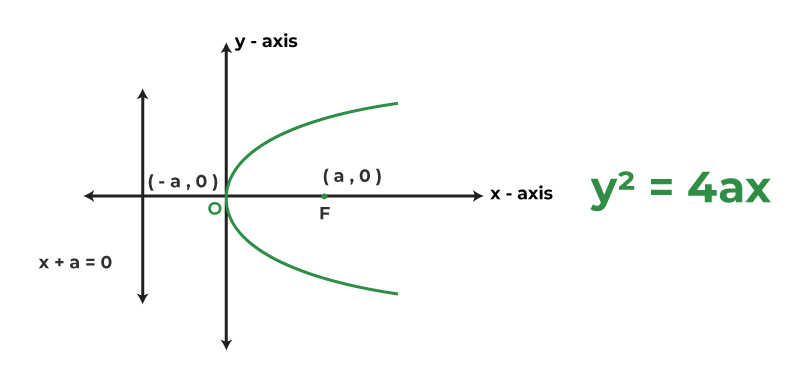
\includegraphics[width=0.6\textwidth]{parabola.png}
\begin{itemize}
    \item Symmetrix about the $x$-axis
    \item Focus at $(a, 0)$
    \item Vertex at $(0, 0)$
\end{itemize}
\subsection{Definition}
\begin{itemize}
    \item The locus of points that are the \textbf{same distance} from a fixed point, $S$, 
    called the \textbf{focus}, and a fixed straight line called the \textbf{directrix}
    \item $\dfrac{\text{distance to foci}}{\text{distance to directrix}} = e = 1$
\end{itemize}
\subsection{Cartesian equation}
\begin{itemize}
    \item $y^2=4ax$ ($a>0$)
\end{itemize}
\subsection{Parametric equation}
\begin{itemize}
    \item $x=at^2$
    \item $y=2at$
    \item $t\in \Rset$
\end{itemize}
\subsection{Eccentricity}
\begin{itemize}
    \item $e=1$
\end{itemize}
\subsection{Directrix}
\begin{itemize}
    \item The directrix has equation $x+a=0$
\end{itemize}
\subsection{Tangents and normals}
\begin{itemize}
    \item $\dfrac{\dy}{\dx} = \frac{1}{t} = \frac{2a}{y}$
    \item Equation of tangent: $ty=x+at^2$ at $P(at^2, 2at)$
    \item Equation of normal: $y+tx=2at+at^3$ at $P(at^2, 2at)$
\end{itemize}

\section{Rectangular hyperbolas}
\subsection{Graph}
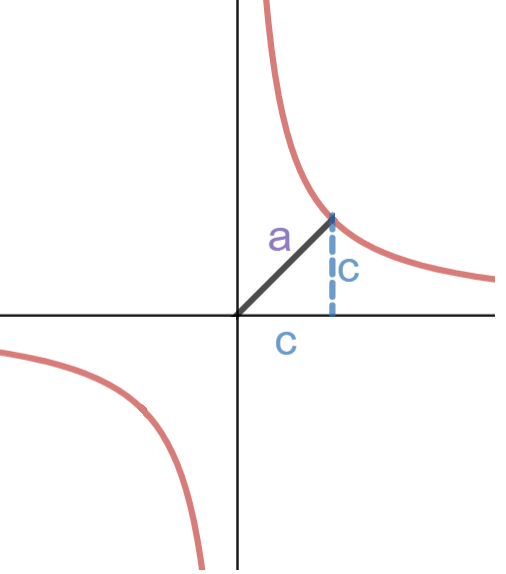
\includegraphics[width=0.3\textwidth]{rectangular_hyperbola.png}
\begin{itemize}
    \item Asymptotes at $x=0$ and $y=0$ ($x$ and $y$-axis)
\end{itemize}
\subsection{Definition}
\begin{itemize}
    \item The locus of points that are the \textbf{same distance} from a fixed point, $S$, 
    called the \textbf{focus}, and a fixed straight line called the \textbf{directrix}
    \item $\dfrac{\text{distance to foci}}{\text{distance to directrix}} = e = 1$
\end{itemize}
\subsection{Cartesian equation}
\begin{itemize}
    \item $xy=c^2$ ($c>0$)
\end{itemize}
\subsection{Parametric equation}
\begin{itemize}
    \item $x=ct$
    \item $y=\frac{c}{t}$
    \item $t \neq 0, t\in\Rset$
\end{itemize}
\subsection{Eccentricity}
\begin{itemize}
    \item $e=\sqrt{2}$
\end{itemize}
\subsection{Directrix}
\begin{itemize}
    \item $x+y=\pm c\sqrt{2}$
\end{itemize}
\subsection{Tangents and normals}
\begin{itemize}
    \item Equation of tangent: $x+t^2y=2ct$ at $P(ct, \frac{c}{t})$
    \item Equation of normal: $t^3x-ty=c(t^4-1)$ at $P(ct, \frac{c}{t})$
\end{itemize}